\section{Supplement: the final windows of the first version}
\label{sec:supplementfinal}

The first version of this paper scored each data set once, on its final window,
with three seeds per trained model. These results come before the rolling
windows of the main text and are kept here for the record.


\begin{table*}[t]
\centering
\caption{\textbf{On M5 the best model depends on the level scored and on the month.} WRMSSE on the four 28-day
windows (lower is better), mean over seeds; seeds per window in the second column. All: the 12 levels together;
Total: the chain total; I$\times$S: item by store. The lowest value in each column is in bold. TimesFM with the
plan has no recorded total. The lift model's April mean includes one failed seed (2.603 overall;
\S\ref{sec:failures}).}
\label{tab:m5}
\footnotesize
\setlength{\tabcolsep}{3.6pt}
\begin{tabular}{lc*{12}{r}}
\toprule
 & & \multicolumn{3}{c}{\textbf{29 Feb to 27 Mar}} & \multicolumn{3}{c}{\textbf{28 Mar to 24 Apr}} & \multicolumn{3}{c}{\textbf{25 Apr to 22 May (practice)}} & \multicolumn{3}{c}{\textbf{23 May to 19 Jun (test)}} \\
\cmidrule(lr){3-5}\cmidrule(lr){6-8}\cmidrule(lr){9-11}\cmidrule(lr){12-14}
\textbf{Model} & \textbf{Seeds} & All & Total & I$\times$S & All & Total & I$\times$S & All & Total & I$\times$S & All & Total & I$\times$S \\
\midrule
World model & 3/3/3/3 & \textbf{0.642} & \textbf{0.398} & 0.851 & \textbf{0.555} & \textbf{0.283} & 0.833 & 0.656 & 0.535 & 0.834 & 0.638 & 0.379 & 0.897 \\
Lift model & 3/3/3/3 & 0.664 & 0.427 & 0.846 & 1.246 & 0.964 & 0.834 & 0.713 & 0.623 & 0.832 & 0.663 & 0.368 & 0.896 \\
LightGBM & 3/3/1/3 & 0.709 & 0.578 & 0.873 & 0.557 & 0.351 & 0.846 & 0.715 & 0.659 & 0.847 & \textbf{0.547} & \textbf{0.247} & 0.905 \\
Graph model & 3/3/3/3 & 0.778 & 0.621 & 0.878 & 0.644 & 0.493 & 0.845 & \textbf{0.641} & \textbf{0.455} & 0.851 & 0.673 & 0.412 & 0.909 \\
TimesFM & 1/1/1/1 & 0.854 & 0.830 & \textbf{0.836} & 0.819 & 0.786 & \textbf{0.828} & 0.896 & 0.930 & \textbf{0.828} & 0.729 & 0.558 & 0.885 \\
TimesFM with the plan & 1/1/1/1 & 0.858 & -- & 0.837 & 0.772 & -- & 0.829 & 0.929 & -- & 0.830 & 0.719 & -- & \textbf{0.883} \\
Seasonal naive & 1/1/1/1 & 0.889 & 0.658 & 1.121 & 0.923 & 0.668 & 1.126 & 0.870 & 0.751 & 1.100 & 0.847 & 0.560 & 1.176 \\
\bottomrule
\end{tabular}
\end{table*}

\begin{table*}[t]
\centering
\caption{\textbf{On the promotion-driven weekly data, models that see the plan lead, and which one leads
changes by category.} WRMSSE on the final 8 weeks (lower is better). World model, lift model and LightGBM:
mean of three seeds, settings fixed on the development windows. TimesFM and TimesFM with the plan: one run each,
added after the final tests. The lift model was run on Frat only. The lowest value in each row and group is in bold.}
\label{tab:finals}
\footnotesize
\setlength{\tabcolsep}{4pt}
\begin{tabular}{l*{10}{r}}
\toprule
 & \multicolumn{5}{c}{\textbf{All levels}} & \multicolumn{5}{c}{\textbf{Item by store}} \\
\cmidrule(lr){2-6}\cmidrule(lr){7-11}
\textbf{Data} & World & Lift & LightGBM & TimesFM & TimesFM+plan & World & Lift & LightGBM & TimesFM & TimesFM+plan \\
\midrule
Frat & 0.681 & 0.714 & \textbf{0.549} & 0.965 & 0.686 & 0.665 & 0.677 & \textbf{0.608} & 0.827 & 0.641 \\
\addlinespace[2pt]
\multicolumn{11}{l}{\itshape Dominick's} \\
Cheese & 0.897 & -- & 0.708 & 0.829 & \textbf{0.545} & 0.715 & -- & 0.702 & 0.792 & \textbf{0.699} \\
Snack crackers & 0.448 & -- & \textbf{0.412} & 0.468 & 0.475 & 0.608 & -- & \textbf{0.596} & 0.640 & 0.614 \\
Soft drinks & \textbf{0.830} & -- & 0.989 & 1.070 & 0.974 & 0.734 & -- & \textbf{0.652} & 0.895 & 0.780 \\
Bottled juice & 0.987 & -- & 0.994 & \textbf{0.940} & 0.990 & 0.816 & -- & \textbf{0.750} & 0.782 & 0.754 \\
Analgesics & \textbf{0.867} & -- & 0.978 & 1.009 & 0.889 & \textbf{0.713} & -- & 0.714 & 0.790 & 0.742 \\
Frozen entrees & 0.485 & -- & \textbf{0.478} & 0.563 & 0.566 & 0.557 & -- & \textbf{0.529} & 0.682 & 0.599 \\
\bottomrule
\end{tabular}
\end{table*}

\begin{table*}[t]
\centering
\caption{\textbf{On the single final windows the ensemble is lowest or within \rcount{finalsgap} of the lowest item by
store on every data set, and the order at the total changes from data set to data set.} WRMSSE on the final
window of each data set (lower is better; on M5 the official test month). One fit (seed~1) per trained model, so the world
model and LightGBM differ slightly from the three-seed means of Tables~\ref{tab:m5} and~\ref{tab:finals}. Bold:
lowest in the group.}
\label{tab:finalsnew}
\footnotesize
\setlength{\tabcolsep}{3pt}
\begin{tabular}{l*{14}{r}}
\toprule
 & \multicolumn{7}{c}{\textbf{Item by store}} & \multicolumn{7}{c}{\textbf{Total}} \\
\cmidrule(lr){2-8}\cmidrule(lr){9-15}
\textbf{Data} & Ens. & World & Lift & LGB & TFM+p & Chr. & TFT & Ens. & World & Lift & LGB & TFM+p & Chr. & TFT \\
\midrule
Cheese & \textbf{0.675} & 0.712 & 0.756 & 0.699 & 0.704 & 0.807 & 0.731 & 0.753 & 1.064 & 0.997 & 0.768 & 0.531 & 1.009 & \textbf{0.522} \\
Snack crackers & \textbf{0.585} & 0.610 & 0.620 & 0.603 & 0.624 & 0.661 & 0.621 & 0.334 & 0.484 & 0.302 & 0.317 & 0.362 & 0.327 & \textbf{0.219} \\
Soft drinks & 0.674 & 0.709 & 0.772 & \textbf{0.655} & 0.780 & 0.912 & 0.849 & 1.065 & \textbf{0.891} & 0.920 & 1.238 & 1.140 & 1.385 & 1.228 \\
Bottled juice & 0.760 & 0.849 & 0.807 & 0.756 & \textbf{0.754} & 0.785 & 0.775 & 1.111 & 1.019 & 1.190 & 1.171 & 1.172 & 1.046 & \textbf{1.015} \\
Analgesics & \textbf{0.710} & 0.712 & 0.714 & 0.716 & 0.742 & 0.802 & 0.770 & 1.236 & 1.186 & 1.280 & 1.407 & 1.149 & 1.454 & \textbf{0.878} \\
Frozen entrees & 0.543 & 0.574 & 0.563 & \textbf{0.530} & 0.599 & 0.692 & 0.557 & 0.454 & 0.423 & \textbf{0.404} & 0.438 & 0.537 & 0.536 & 0.414 \\
Frat & \textbf{0.604} & 0.671 & 0.662 & 0.613 & 0.644 & 0.856 & 0.702 & 0.586 & 0.681 & 0.698 & \textbf{0.523} & 0.677 & 1.222 & 0.818 \\
M5 & \textbf{0.881} & 0.896 & 0.896 & 0.905 & 0.883 & 0.899 & -- & \textbf{0.240} & 0.363 & 0.424 & 0.245 & 0.556 & 1.007 & -- \\
\bottomrule
\end{tabular}
\end{table*}


The first version scored each data set once, on its final window, and its
findings stand: on M5 the most accurate model depended on the level and the
month (Table~\ref{tab:m5}), and on Dominick's and Frat on the category
(Table~\ref{tab:finals}). On M5, TimesFM given only history was the most
accurate single model item by store in all four months (\mTfmTestIxs{} on the
test month, against \mWorldTestIxs{} for the world model and \mLgbTestIxs{} for
LightGBM), while the plan-aware models were far more accurate at the totals. The
official test month was the only one of four in which LightGBM was the most
accurate over all levels (\mLgbTestOverall{} against \mWorldTestOverall), so a
comparison on that month alone would have ranked it first. Run on the final
windows (Table~\ref{tab:finalsnew}), the ensemble is lowest or within
\rcount{finalsgap} of the lowest item by store on every data set, which agrees
with the rolling windows.

\begin{figure*}[t]
\centering
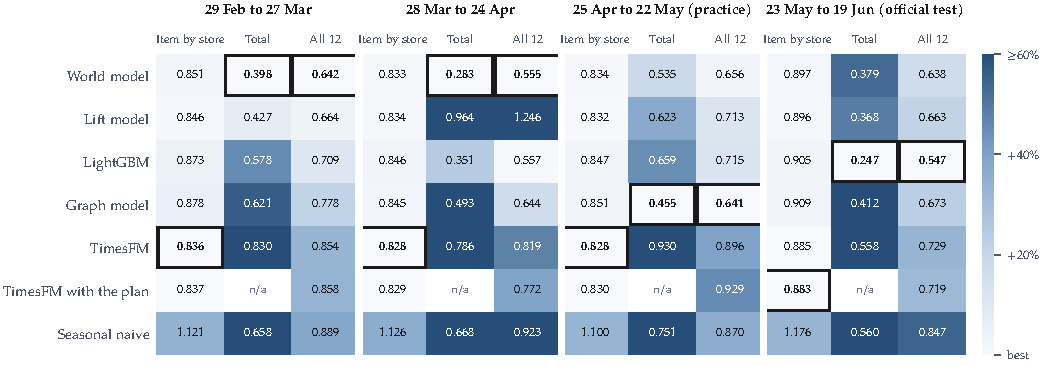
\includegraphics[width=\textwidth]{figs/fig_m5_heat.pdf}
\caption{\textbf{On the M5 final windows, TimesFM from history alone had the
lowest item-by-store error of the single models in every month; at the total and
over all levels the plan-aware models did, and which one changed by month.}
WRMSSE of every single model, four windows, three levels; cell shade: how far
above the lowest value in its column (white: the lowest, outlined). Trained
models: mean of three seeds. The lift model's April mean includes one failed
seed (\S\ref{sec:dropped-first}).}
\label{fig:m5heat}
\end{figure*}

\paragraph{How much the plan matters}
On M5, where prices rarely change, giving TimesFM the plan changed its
item-by-store error by at most 0.002 in any month. On Dominick's, where promoted
weeks carry \promoShareLo\% to \promoShareHi\% of a category's units, TimesFM
without the plan forecast \promoTfmLo\% to \promoTfmHi\% of promoted-week sales
and with it \promoTfmPlanLo\% to \promoTfmPlanHi\%
(Figure~\ref{fig:planarrows}a). The trained plan-aware models also fell short in
promoted weeks: the world model forecast \promoWorldLo\% to \promoWorldHi\% of
promoted-week sales and LightGBM \promoLgbLo\% to \promoLgbHi\%.

\begin{figure*}[t]
\centering
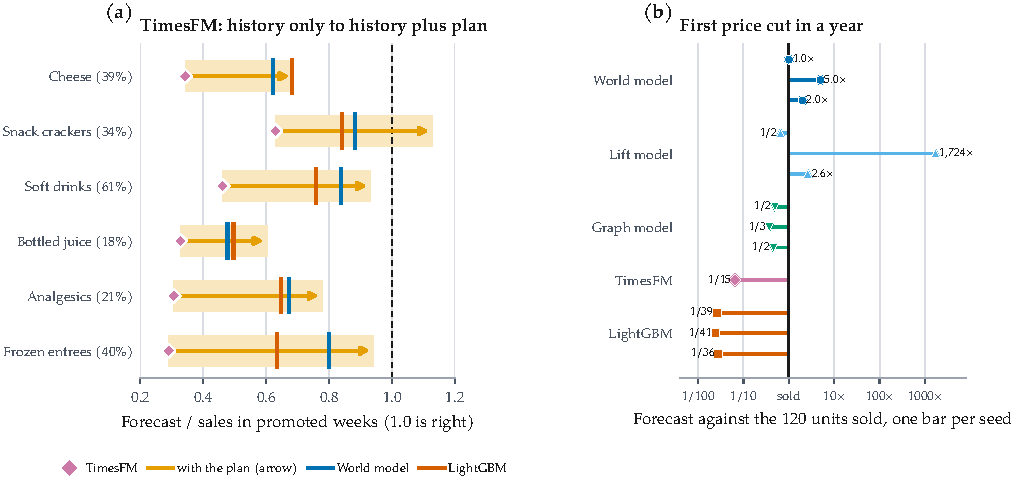
\includegraphics[width=\textwidth]{figs/fig_plan_arrows.pdf}
\caption{\textbf{Given the plan, TimesFM closes most of its promoted-week
shortfall; for a price cut history has not shown, plan-aware models respond and
history-only models do not.} \textbf{(a)} Forecast against sales in the promoted
weeks of the final 8 weeks, by Dominick's category (promoted weeks' share of the
category's units in brackets): TimesFM from history alone (diamond) to TimesFM
with the plan (arrow head), with the world model and LightGBM (ticks). \textbf{(b)}
HOUSEHOLD\_1\_146 in the four M5 stores where it had its first price cut in a year
(5.98 to 4.50 for one week) inside the April window: each seed's forecast over
the 28 days against the \cutSold{} units sold, log scale.}
\label{fig:planarrows}
\end{figure*}

\paragraph{First-time price cuts}
In the April M5 window, HOUSEHOLD\_1\_146 had sold almost nothing for a year at
5.98, then sold \cutSold{} units in four stores over a window that held a
one-week cut to 4.50 (Figure~\ref{fig:planarrows}b). Models working from history
forecast almost nothing: LightGBM \cutLgb{} units across seeds, TimesFM
\cutTfm. The world model, which reads the cut through its plan, forecast
\cutWorld; the graph model \cutGraph; the lift model \cutLift. How large the
response should be is not fixed by the data: the world-model seeds differ by a
factor of five, and one lift-model seed forecast over 200,000 units.


\subsection{What the first version tried and dropped}
\label{sec:dropped-first}

\begin{table*}[t]
\centering
\caption{\textbf{Every change and comparison model that did not become a default.} Overall WRMSSE unless
stated; ``against'' gives the default it was compared with on the same window. dev.: development windows before
the final 8 weeks. Practice: the M5 window 25 April to 22 May 2016. Each row is a section of
\texttt{results/README.md} with its run folders.}
\label{tab:ledger}
\footnotesize
\begin{tabular}{p{0.30\textwidth}p{0.28\textwidth}p{0.34\textwidth}}
\toprule
\textbf{Change or model} & \textbf{Where tested} & \textbf{Result} \\
\midrule
Twice the training steps & Dominick's (6) and Frat, dev., 3 seeds & Better in 2, worse in 3, level or mixed in 2 \\
Weekday as seven inputs & M5 practice, seed 1 & 0.653 against 0.646 \\
Event kinds (with weekday) & M5 practice, seed 1 & 0.646 against 0.646 \\
60,000 training steps & M5 practice, seed 1 & 0.642 against 0.646; gain below seed range 0.029 \\
Item level against past-year level & M5 practice, seed 1 & 0.680 against 0.646 \\
Totals term in the loss & Dominick's analgesics, dev. & 0.819 against 0.683; total 8\% under \\
Negative binomial likelihood & Frat, analgesics, dev. & Level \\
Plan split, latent check, near-week weighting & Frat, dev., 5 seeds & 0.417 to 0.427 against 0.408 \\
Own forecast fed into the roll-forward & Dominick's (6), dev. & Worse overall in 4 of 6 \\
Item role labels & Dominick's (6), dev. & No effect on LightGBM; snack crackers 2.422 for the world model \\
Averaging three fits & M5 practice, seed 1 & 0.665 against 0.656 (kept on Dominick's) \\
Graph model over product attributes & M5, four windows, 3 seeds & Level with LightGBM item by store \\
TimesFM, median output & M5, four windows & Overall 1.71 to 1.88; totals 27\% to 31\% under \\
Lift model (no roll-forward) & M5, four windows, 3 seeds & One seed failed in April (2.603) \\
\bottomrule
\end{tabular}
\end{table*}


\paragraph{A lift-model seed that broke on five series}
In the April M5 final window, lift-model seed 2 scored \mLiftAprSeedBOverall{}
over all levels against \mLiftAprSeedAOverall{} and \mLiftAprSeedCOverall{} for
seeds 1 and 3, and forecast \liftSeedTwoForecast{} units against
\liftSeedTwoSold{} sold. Five item-store series hold all of the excess, each with
its first price cut in a year inside the window; the seed read the cuts as lifts
up to the model's bound. Item by store, weighted by dollar sales, the failure is
invisible (\mLiftAprIxs); at the totals it dominates. The world model did not
fail on these series in any seed.

\begin{figure*}[t]
\centering
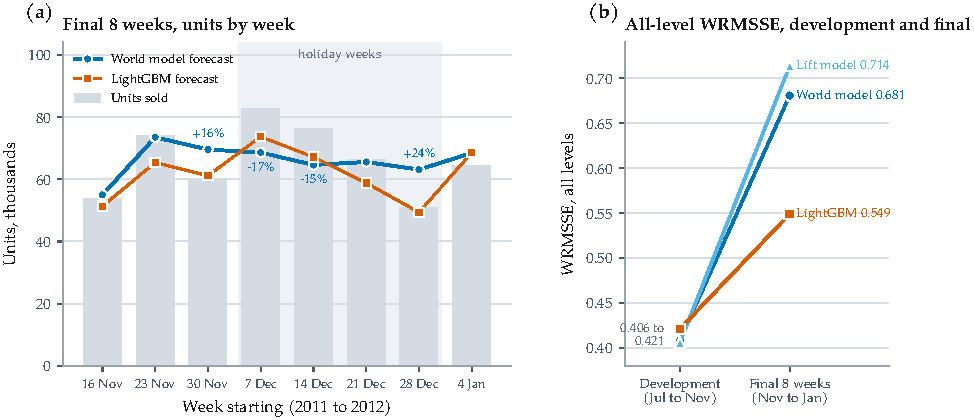
\includegraphics[width=\textwidth]{figs/fig_frat_story.pdf}
\caption{\textbf{On the Frat final window the world model got the 8-week total
right and missed the holiday shape, which the development windows did not
contain.} \textbf{(a)} Units sold each week of the final window over all
item-stores (bars), and the weekly forecasts of the world model and LightGBM,
three seeds averaged; labels: the world model's largest weekly misses.
\textbf{(b)} All-level WRMSSE on the development windows and on the final 8 weeks.}
\label{fig:fratstory}
\end{figure*}

\paragraph{Frat holiday weeks}
On the Frat development windows the world model, lift model and LightGBM were
level (0.406 to 0.421). On the final 8 weeks the world model fell to
\fWorldFratOverall{} against \fLgbFratOverall{} for LightGBM. The final weeks
are the holiday period, which the development windows did not contain
(Figure~\ref{fig:fratstory}); the world model's 8-week total is right (forecast
against sales \fWorldFratFa) but it is 15\% to 17\% under in the two December
peak weeks. LightGBM, with week-of-year and month inputs and the previous
holiday season in its training data, follows that shape more closely.

\paragraph{TimesFM's default output}
TimesFM's default point forecast is the median. For an item that sells nothing
on most days the median is near zero while the mean is not, so the median
forecast is 27\% to 31\% below M5 totals in every month. The mean output, used
throughout, does not have the problem.

